\documentclass[a4paper, 12pt]{article}
\usepackage{geometry}
\geometry{a4paper,
total={170mm,257mm},left=2cm,right=2cm,
top=2cm,bottom=2cm}

\usepackage{mathtext}
\usepackage{amsmath}
\usepackage[utf8]{inputenc}
\usepackage[english,russian]{babel}
\usepackage{graphicx, float}
\usepackage{tabularx, colortbl}
\usepackage{caption}
\usepackage{subfigure}
\usepackage{wrapfig}
\captionsetup{labelsep=period}

\newcommand{\parag}[1]{\paragraph*{#1:}}
\DeclareSymbolFont{T2Aletters}{T2A}{cmr}{m}{it}
\newcounter{Points}
\setcounter{Points}{1}
\newcommand{\point}{\arabic{Points}. \addtocounter{Points}{1}}
\newcolumntype{C}{>{\centering\arraybackslash}X}

\author{Калинин Даниил, Б01-110}
\date{\today}
\title{Лабораторная работа 1.2.5\\Измерение прецессии уравновешенного гироскопа}

\begin{document}
\maketitle

\parag {Цель работы}
Исследовать вынужденную прецессию гироскопа, установить зависимость скорость вынужденной прецессии от момента сил, действующих на ось гироскопа, определить скорость вращения ротора гироскопа и сравнить ее со скоростью, рассчитанной по скорости прецессии.

\parag {В работе используются}
гироскоп в кардановом подвесе, секундомер, набор грузов, отдельный ротор гироскопа, цилиндр известной массы, крутильный маятник, штангенциркуль, линейка.

\parag {Теоритическая справка} ~\\

Основные уравнения движения твердого тела можно записать в виде:

\begin{equation}
	\frac{d\vec{P}}{dt} = \vec{F}
	\label{eq:center_of_mass}
\end{equation}

\begin{equation}
	\frac{d\vec{L}}{dt} = \vec{M}
	\label{eq:moments_equation}
\end{equation}

Формула (\ref{eq:center_of_mass}) выражает закон движения центра масс, а формула (\ref{eq:moments_equation}) -- уравнение моментов, действующих на тело. Двух данных уравнений достаточно для описания состояния твердого тела.

Если сила $\vec{F}$ не зависит от угловой скорости вращения тела, а момент $\vec{M}$ от скорости поступательного движения тела, то уравнения (\ref{eq:center_of_mass}) и (\ref{eq:moments_equation}) можно рассматривать независимо друг от друга. В данной работе рассматривается только задача о вращении твердого тела.

Момент импульса твердого тела можно вычислить, используя формулу:

\begin{equation}
	\vec{L} = \vec{i}I_{x}\omega_{x} + \vec{j}I_{y}\omega_{y} + \vec{k}I_{z}\omega_{z},
\end{equation}

где $ I_{x},I_{y},I_{z} $ -- главные моменты инерции тела, $ \omega_{x}, \omega_{y}, \omega_{z} $ -- компоненты вектора угловой скорости  $\vec{\omega} $.

Быстро вращающееся тело, для которого:

	$$I_{z}\omega_{z} \gg I_{x}\omega_{x}, I_{y}\omega_{y}$$

принято называть \textit{гироскопом}. Гироскоп называется уравновешенным, если его центр масс неподвижен.

В силу (\ref{eq:moments_equation}), приращение момента импулься определяется интегралом:
\begin{equation}
	\Delta\vec{L} =  \int\vec{M}\\,dt
	\label{eq:integral_for_increment}
\end{equation}

Если момент внешних сил действует в течение короткого промежутка времени, из формулы (\ref{eq:integral_for_increment}) следует, что приращение $\vec{L}$ момента импулься значительно меньше самого момента импульса, т.е:

\begin{equation}
	\left| \Delta\vec{L} \right| \ll \left| \vec{L} \right|.
\end{equation}

Благодаря этому, гироскоп приобретает очень большую устойчивость, вызванную его быстрым вращением.

Если гироскоп уравновешен, то суммарный момент сил, действующих на него, равен 0. В таком случае, гироскоп не будет изменять своего положения в пространстве. Если на гироскоп в течение длительного времени будет действовать некоторый момент сил, отличный от нуля, то, согласно (\ref{eq:moments_equation}) гироскоп придет в движение. Мы не будем рассматривать действие моментов сил, которые вызовут ускорение или замедление гироскопа (т.е. моментов сил, которые не изменяют положения оси вращения гироскопа). Рассмотрим действия моментов сил, которые изменяют положение оси вращения гироскопа.

\begin{wrapfigure}[19]{r}{0.4\textwidth}
	\vspace{-2.5ex}
	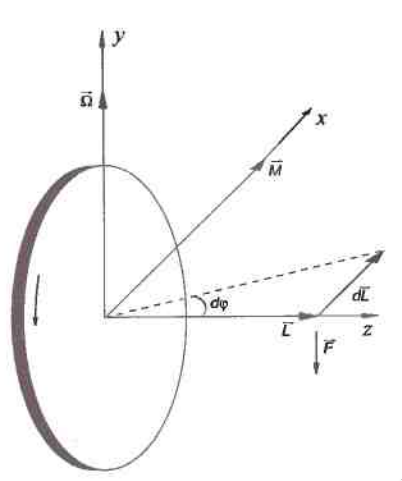
\includegraphics[width = 0.35\textwidth]{flywhell.png}
	\caption{Маховик.}
	\label{fig:flywheel}
\end{wrapfigure}

Рассмотрим маховик, вращающийся вокруг оси z. (Рис. \ref{fig:flywheel}). Будем считать, что 
$$ \omega_{z} = \omega_{0},\qquad \omega_{x} = \omega_{y} = 0.$$

Пусть ось вращения повернулась в плоскости \textit{zx} по направлению в оси \textit{x} на бесконечно малый угол $d\varphi$. Такой поворот означает добавочное вращение маховика вокруг оси \textit{y}, так что 
$$ d\varphi = \Omega\,dt, $$
где $ \Omega $ -- угловая скорость такого вращения. Будем предполагать, что
\begin{equation}
	L_{\Omega} \ll L_{\omega_{0}}
	\label{eq:condition_for_rotate}
\end{equation}

Это означает, что момент импульса маховика, равный $I_{z}\omega_{0}$ до приложения внешних сил, только повернется в плоскости \textit{zx} по направлению к оси \textit{x} не изменяя своей величины. Таким образом,

\begin{equation}
	\left|d\vec{L}\right| = Ld\varphi = I\Omega\,dt
	\label{eq:increment_moment_of_impulse}
\end{equation}


Записывая выражение (\ref{eq:increment_moment_of_impulse}) в виде векторного произведения, получаем:

\begin{equation}
	\frac{d\vec{L}}{dt} = \vec{\Omega} \times \vec{L}
\end{equation}

Окончательно, используя (\ref{eq:moments_equation}), получаем:

\begin{equation}
	\vec{M} = \vec{\Omega} \times \vec{L}
	\label{eq:rotation_by_moments_of_force}
\end{equation}

Формула (\ref{eq:rotation_by_moments_of_force}) справедлива, если выполнено условие (\ref{eq:condition_for_rotate}).
Данная формула позволяет определить, момент сил $ \vec{M}, $ который нужно приложить к маховику, чтобы вызвать вращение маховика с угловой скоростью $\vec{\Omega}$.

Под действием момента внешних сил $\vec{M}$ ось гироскопа медленно вращается вокруг оси \textit{y} с угловой скоростью $\vec{\Omega}$. Такое движение называют \textit{прецессией гироскопа}.

Для изучения регулярной прецессии уравновешенного гироскопа к его оси подвешивают дополнительные грузы. Это смещает общий центр масс и создает момент сил тяжести, вызывающий прецессию. Скорость прецессии в этом случае может быть найдена по формуле:

\begin{equation}
	\Omega = \frac{mgl}{I_{z}\omega_{0}},
	\label{eq:teor_equation_omega}
\end{equation} 
где m -- масса груза, l -- расстояние от центра карданова подвеса до точки крепления груза на оси гироскопа. (Рис. \ref{fig:facility})

Для выполнения работы используется гироскоп (Рис. \ref{fig:facility}), закрепленный в карданном подвесе (Рис. \ref{fig:Cardan_suspension}).


\begin{figure}[ht!]  
	\vspace{-1ex} 
	\centering 
	\subfigure[]{
		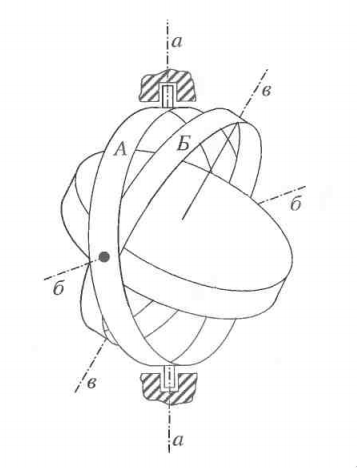
\includegraphics[width=0.29\linewidth]{cardan.png} 	
			\label{fig:Cardan_suspension}}  
	\hspace{4ex}
	\subfigure[]{
		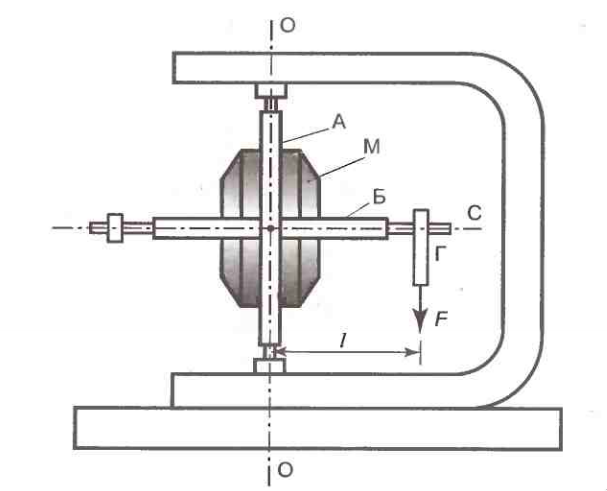
\includegraphics[width=0.45\linewidth]{gyro.png} 
			\label{fig:facility} }  
	\caption{а) Гироскоп, закрепленный в карданном подвесе. б) Схема устройства гироскопа.}
\end{figure}

Ротором гироскопа (Рис. \ref{fig:facility}) является ротор электромотора М. Кожух мотора скреплен с кольцом Б (Рис. \ref{fig:Cardan_suspension}). Мотор с кольцом Б может вращаться в кольце А вокруг горизонтальной оси бб, которое может вращаться относительно оси аа. Рычаг С направлен по оси симметрии ротора. на рычаг подвешивают грузы Г.


\parag {Ход работы} ~\\
\point Запишем погрешности измерительных приборов в таблицу \ref{tabl:inaccs}.

\begin{table}[H]
    \centering
    \begin{tabular}{|l|l|l|}
    \hline 
           & Прибор         & Погрешность          \\ \hline
    1      & Линейка        & $\sigma = 0.5 $ мм.  \\ \hline
    2      & Штангенциркуль & $\sigma = 0.05$ мм.  \\ \hline
    3      & Секундомер     & $\sigma = 0.5 $ с.    \\ \hline
    \end{tabular}
	\caption{Погрешности}
    \label{tabl:inaccs}
\end{table}

\point Измерим период прецессии оси гироскопа. Для этого будем отклонять ось гироскопа примерно на 5-6 градусов выше горизонтальной плоскости, вешать груз и, следя за тем, чтобы ось гироскопа опустилась ниже горизонтальной плоскости примерно на тот же угол, на который мы ее отклонили, измерим целое число периодов. Полученные значения, а также расчитанные периоды прецессии занесем в таблицу \ref{tabl:data_row}

\begin{table}
    \centering
    \begin{tabular}{|l|l|l|}
    \hline
    Количество оборотов & Полное время, c. & Период прецессии, c.   \\ \hline
    \multicolumn{3}{|c|}{$m = 142 гр.$}                     \\ \hline
    3   &   $221 \pm 0.5$   &   $73.7$                      \\ \hline
    3   &   $219 \pm 0.5$   &   $73.0$                      \\ \hline
    3   &   $220 \pm 0.5$   &   $73.3$                      \\ \hline
    3   &   $221 \pm 0.5$   &   $73.7$                      \\ \hline

    \multicolumn{3}{|c|}{$m = 179 гр.$}                     \\ \hline
    3   &   $174 \pm 0.5$   &   $58.0 $                     \\ \hline
    4   &   $232 \pm 0.5$   &   $58.0 $                     \\ \hline
    4   &   $232 \pm 0.5$   &   $58.0 $                     \\ \hline
    4   &   $233 \pm 0.5$   &   $58.25$                     \\ \hline
    
    \multicolumn{3}{|c|}{$m = 220 гр.$}                     \\ \hline
    5   &   $236 \pm 0.5$   &   $47.2$                      \\ \hline
    5   &   $232 \pm 0.5$   &   $46.4$                      \\ \hline
    5   &   $235 \pm 0.5$   &   $47.0$                      \\ \hline
    5   &   $234 \pm 0.5$   &   $46.8$                      \\ \hline

    \multicolumn{3}{|c|}{$m = 274 гр.$}                     \\ \hline
    6   &   $262 \pm 0.5$   &   $43.7$                      \\ \hline
    6   &   $264 \pm 0.5$   &   $44.0$                      \\ \hline
    6   &   $266 \pm 0.5$   &   $44.3$                      \\ \hline
    6   &   $265 \pm 0.5$   &   $44.2$                      \\ \hline
    
    \multicolumn{3}{|c|}{$m = 342 гр.$}                     \\ \hline
    8   &   $242 \pm 0.5$   &   $30.25$                     \\ \hline
    8   &   $246 \pm 0.5$   &   $30.75$                     \\ \hline
    8   &   $245 \pm 0.5$   &   $30.6 $                     \\ \hline
    8   &   $247 \pm 0.5$   &   $30.9 $                     \\ \hline

    \end{tabular}
	\caption{Результаты иземерений периодов прецессии оси гироскопа}
    \label{tabl:data_row}
\end{table}

\point Усредним полученные для разных грузов периоды, расчитаем погрешности измерений результат занесем в таблицу \label{tabl:data_2}

\begin{table}
    \centering
    \begin{tabular}{|l|l|l|l|l|l|}
    \hline
    $m_г$, гр. & $\bar{T}$, с. & $\sigma_{сист.}$ &  $\sigma_{случ.}$ &  $\sigma_{\bar{T}}$ & $\varepsilon_{\bar{T}}$ \\ \hline
    142 & 73.42 & 0.5 & 0.29 & 0.58 & 0.008 \\ \hline
    179 & 58.06 & 0.5 & 0.11 & 0.51 & 0.009 \\ \hline
    220 & 46.85 & 0.5 & 0.30 & 0.58 & 0.012 \\ \hline
    274 & 44.05 & 0.5 & 0.23 & 0.55 & 0.012 \\ \hline
    342 & 30.62 & 0.5 & 0.24 & 0.56 & 0.018 \\ \hline

    \end{tabular}
	\caption{Усредненное значение периода прецессии, а также погрешности измерения периода прецессии}
    \label{tabl:mean_periods}
\end{table}

Как можно заметить из таблицы \ref{tabl:mean_periods}, величина относительной погрешности измерения периода прецессии достаточно мала. определим по полученным данным величину $\Omega$. Для этого воспользуемся формулой:

\begin{equation}
	\Omega = \frac{2\pi n}{t_{\text{полн}}}
	\label{eq:definition_Omega}
\end{equation} 
	
Применив формулу \ref{eq:definition_Omega} к данным таблицы \ref{tabl:mean_periods} и занесем результат в таблицу \ref{tabl:first_experimental_Omega}. На основе данных таблицы построим график, изображенный на рисунке \ref{fig:graphic_Omega_moment}.

\begin{table}
    \centering
    \begin{tabular}{|l|l|l|l|l|l|}
    \hline
    Масса груза, г. & 142 & 179 & 220 & 274 & 342 \\ \hline
    Cкорость прецессии, рад / с. & 0.0856 & 0.1082 & 0.1341 & 0.1426 & 0.2052 \\ \hline
    \end{tabular}
	\caption{Значения угловой скорости прецессии для различных грузов}
    \label{tabl:first_experimental_Omega}
\end{table}

\begin{figure}[h!]
	\begin{center}
		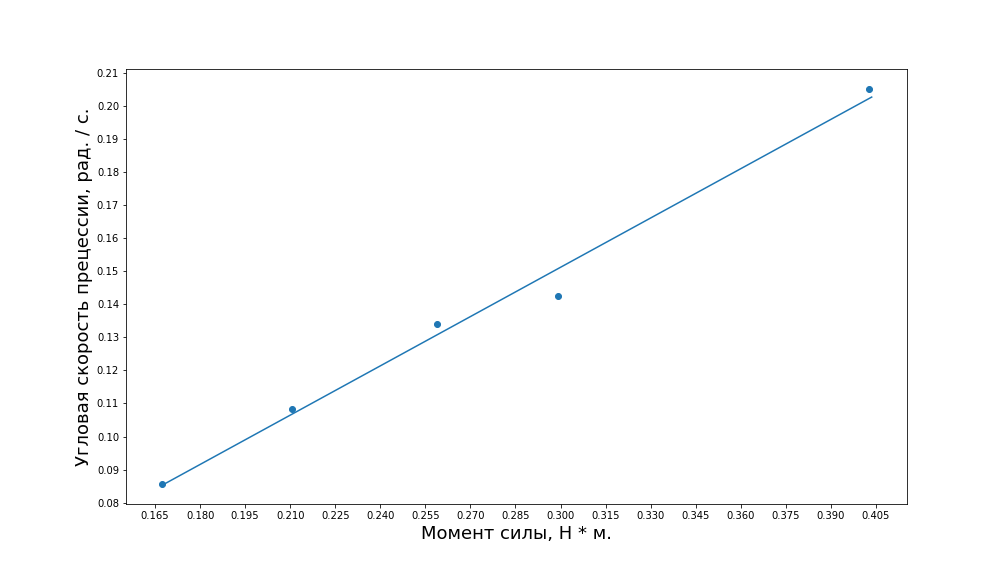
\includegraphics[width = 0.95\textwidth]{Omega-ForceMoment.png}
		\caption{График зависимости $\Omega(M)$}
		\label{fig:graphic_Omega_moment}
	\end{center}
\end{figure}

\point Теперь измерим момент инерции ротора гироскопа методом крутильных колебаний. Для определения момента инерции ротора гироскопа используем формулу:

\begin{equation}
	I_{\text{ротора}}= I_{\text{ц}}\frac{T_{\text{ротора}}^2}{T_{\text{ц}}^2},
	\label{eq:moment_measuring_equation}
\end{equation}
где $I_{\text{ц}}$ -- момент инерции цилиндра, $T_{\text{ротора}}$ -- период крутильных колебаний ротора гироскопа, $T_{\text{ц}}$ -- период крутильных колебаний цилиндра.

Произведем измерение данных величин.
Измерения периодов колебаний будем проводить, отсчитывая 16 полных колебаний. Полученные результаты занесем в таблицу \ref{tabl:results_of_measuring}

\begin{table}[h!]
	\centering
		\begin{tabular}{|l|l|l|}
			\hline
			Величина 			 & значение & $\sigma$    \\ \hline
			$16T_{0}$, c  		 & 51.7     & 0,1         \\ \hline
            $16T_{\text{ц}}$, c  & 65.33    & 0,1         \\ \hline
			$M_{\text{ц}}$, г    & 1617,2   & 0,1         \\ \hline
			$R_{\text{ц}}$, мм   & 40       & 0,25        \\ \hline
		\end{tabular}
		\caption{Результаты измерения периода колебаний ротора и цилиндра на крутильном маятнике}
		\label{tabl:results_of_measuring}
\end{table}

Используя формулу \ref{eq:moment_measuring_equation} и данные таблицы \ref{tabl:results_of_measuring} получим итоговые значения, занесенные в таблицу \ref{tabl:results_of_measuring_moment}.

Величины $\varepsilon_{T}, \varepsilon_{I_{\text{ц}}}, \varepsilon_{I_{0}}$ рассчитываются по следующим формулам:

\begin{equation}
	\varepsilon_{T} = \frac{\sigma_{T}}{T}
\end{equation}	

\begin{equation}
	\varepsilon_{I_{\text{ц}}} = \left(\frac{\sigma_{M}}{M}\right) + 2\left(\frac{\sigma_{R}}{R}\right)
\end{equation}	

\begin{equation}
	\varepsilon_{I_{0}} = \varepsilon_{I_{\text{ц}}} + \varepsilon_{T_{0}} + \varepsilon_{T_{\text{ц}}}
\end{equation}

\begin{table}[h!]
	\centering
	\begin{tabular}{|c|c|c|c|}
		\hline
		Величина           & Значение       & $\sigma$      & $\varepsilon$     \\ \hline
		$T_{0}, c$         & 3,23           & 0,003         & 0,001             \\ \hline
		$T_{\text{ц}}, c$  & 4,08           & 0,003         & 0,001             \\ \hline
		$I_{\text{ц}}, \text{кг}\cdot \text{м}^{2}, \cdot 10^{-4}$  & 12,9  & 0,2 & 0,013 \\ \hline
		$I_{\text{0}}, \text{кг}\cdot \text{м}^{2}, \cdot 10^{-4}$  & 6,6   & 0,1 & 0,017 \\ \hline
	\end{tabular}
	\caption{Результаты измерений момента инерции ротора гироскопа}
	\label{tabl:results_of_measuring_moment}
\end{table}

В итоге, полученное значение момента инерции ротора цилиндра:

\begin{equation}
	I_{0} = \left(6,6 \pm 0,1 \right) \cdot 10^{-4}\quad \text{Кг} \cdot \text{м}^{2}
	\label{eq:moment_of_inertion_result}
\end{equation} 

Используя величину \ref{eq:moment_of_inertion_result} и формулу \ref{eq:teor_equation_omega} определим величины угловой скорости для каждого из грузов. Значения занесем в таблицу \ref{tab:teor_result_Omega_for_diffrent_frequency}.

\begin{table}[h!]
	\centering
		\begin{tabular}{|c|c|c|c|c|c|}
			\hline
			\multicolumn{6}{|c|}{$\nu=410$Гц}                                       \\ \hline
			$m_г$           & 142       & 179       & 220       & 274       & 342   \\ \hline
			$\Omega$, рад/с & 0.084     & 0.106     & 0.131     & 0.163     & 0.203 \\ \hline
		\end{tabular}
		\caption{Значение угловых скоростей прецессии оси гироскопа в зависимости от груза}
		\label{tab:teor_result_Omega_for_diffrent_frequency}
\end{table}

\begin{figure}[h!]
	\begin{center}
		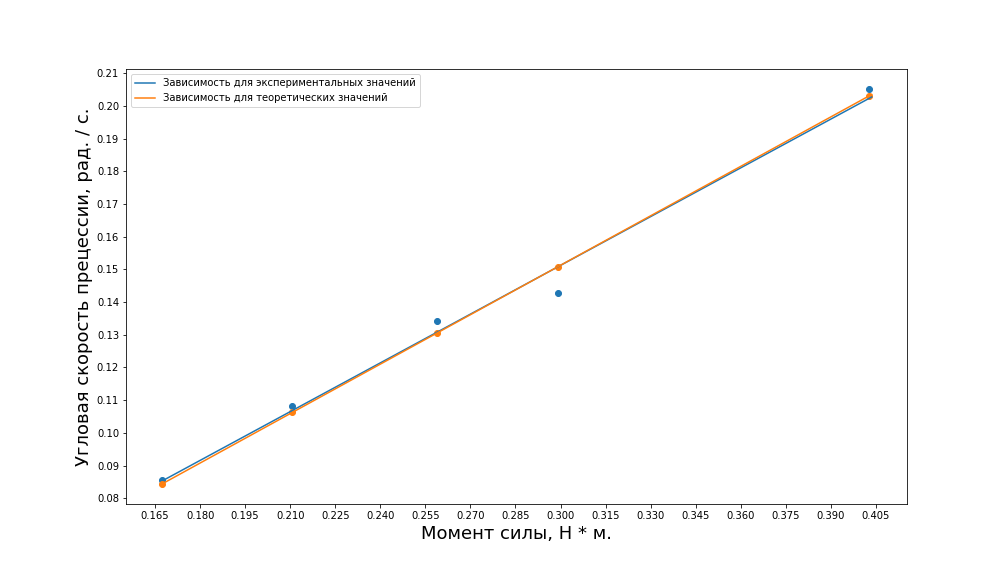
\includegraphics[width = \textwidth]{Omega-Counted.png}
		\caption{Графики зависимости $\Omega(M)$ для разлличных данных}
		\label{fig:diffrent_dependence_Omega}
	\end{center}
\end{figure}

\point Определим моменты сил трения в оси карданного подвеса. 


Для определения скорости прецессии используем формулу:
\begin{equation}
	\Omega_{\text{верт}} = \frac{2\alpha}{t_{all}}
	\label{eq:Omega_vertical}
\end{equation}
где $t_{all}$ -- время, за которое произошло опускание, $\alpha$ -- начальный угол, на который отклонена ось гироскопа от горизонтальной плоскости.

В качестве времени возьмем среднее значении времен, используемых для определения периодов регулярной прецессии
Кроме того, определим значения угла $\alpha$, на который изначально отклонялась ось гироскопа при своем вращении.

Значение времени: $t = 254 $с;

Величину момента сил трения можно определить по следующей формуле:

\begin{equation}
	M_{F_{\text{трения}}} = 2\pi\Omega I_{0}\omega_{z}
\end{equation}

Используя формулу $\ref{eq:Omega_vertical}$, получаем:

\begin{equation}
	M_{F_{\text{трения}}} = \frac{4\pi I_{0}\omega_{z}\arctan\left(\frac{\Delta h}{l}\right)}{t_{\text{полн}}}
	\label{eq:moment_of_force_sopr}
\end{equation}

Используя формулу \ref{eq:moment_of_force_sopr} и полученные ранее значения входящих в нее величин, можем оценить величину момента сил трения, возникающих в оси карданного подвеса:

\begin{equation}
	M_{F_{\text{трения}}} = 2,2 \cdot 10^{-4} \quad\text{Н}\cdot\text{м}
\end{equation}

Определим погрешность полученного результата. 

\begin{equation}
	\sigma_{M} = \sqrt{\varepsilon_{\alpha}^{2} + \varepsilon_{I_{0}}^{2} + \varepsilon_{\omega_{z}}^{2} + \varepsilon_{t_{\text{полн}}}^{2}}
\end{equation}

\begin{equation}
	\sigma_{\alpha} = \frac{\partial \alpha}{\partial \frac{\Delta h}{l}} = \frac{\sigma_{\frac{\Delta h}{l}}}{1 + \frac{\Delta h}{l}}
\end{equation}

В итоге:

\begin{equation}
	M = (2,2 \pm 0,3)\cdot 10^{-4}\quad \text{Н}\cdot\text{м}
\end{equation}

\point Сравним полученные результаты 
В итоге, в ходе выполнения работы были получены следующие результаты:

Значения $\Omega$ представлены в таблице \ref{tab:final_table};

\begin{table}[h!]
\centering
\begin{tabular}{|c|c|}
\hline
$\Omega_{\text{теоретическая}}$, рад/с & $\Omega_{\text{экспериментальная}}$, рад/с \\ \hline
0.086 & 0.084 \\ \hline
0.108 & 0.106 \\ \hline
0.134 & 0.131 \\ \hline
0.143 & 0.151 \\ \hline
0.205 & 0.203 \\ \hline
\end{tabular}
\caption{Значения угловой скорости оси маятника во время прецессии определенные теоретически и экспериментально}
\label{tab:final_table}
\end{table}
 
Значение момента инерции ротора гироскопа: $I_{0} = \left(6,6 \pm 0,1 \right) \cdot 10^{-4}\quad \text{Кг} \cdot \text{м}^{2}$;

Значение момента сил трения в оси карданного подвеса : $M = (2,2 \pm 0,5)\cdot 10^{-4}\quad \text{Н}\cdot\text{м}$

\parag {Заключение} ~\\
В работе были определены величины, описывающие регулярную прецессию гироскопа, закрепленого в карданном подвесе. На практике были подтверждены зависимости, используемые в данной работе. Была достигнута приемлемая точность,  $\varepsilon_{M_{F_{\text{трения}}}} = 0,14$)

\end{document}
